% Compilar com: latexmk -lualatex I1-covariance__covinf.tex
% Tabelas e números em tab/ são gerados por ../../info_covariance_tex.py a partir do manifesto de info_covariance.py.
% Não editar números à mão: regenerar (DESIGN_SYSTEM 2.08).
\documentclass[11pt,a4paper]{article}
\usepackage[margin=2cm]{geometry}
\usepackage{fontspec}
\usepackage{unicode-math}
\setmainfont{Latin Modern Roman}
\setmathfont{Latin Modern Math}
\usepackage[brazil]{babel}
\usepackage{booktabs,tabularx,array,graphicx,float,longtable}
\usepackage{enumitem}
\usepackage{xurl}
\usepackage[colorlinks=true,linkcolor=blue!50!black,urlcolor=blue!50!black,citecolor=blue!50!black]{hyperref}
\usepackage{xcolor}
\setlength{\parindent}{0pt}
\setlength{\parskip}{0.5em}
\newcolumntype{Y}{>{\raggedright\arraybackslash}X}
\newcommand{\arq}[1]{\texttt{\nolinkurl{#1}}}
\newcommand{\caixa}[2]{\par\noindent\colorbox{#1}{\parbox{\dimexpr\linewidth-2\fboxsep}{#2}}\par}
% generated by info_covariance_tex.py from I1-covariance__covinf__learnphob.json; do not edit
\newcommand{\valU}{1{,}48}
\newcommand{\valS}{0{,}025}
\newcommand{\valNbins}{594}
\newcommand{\valNclasses}{11}
\newcommand{\valNsets}{7}
\newcommand{\valNcmp}{64}
\newcommand{\valNphobos}{54}
\newcommand{\valRhoMin}{0{,}95}
\newcommand{\valRhoMax}{1{,}00}
\newcommand{\valResMin}{0{,}6}
\newcommand{\valResMax}{1{,}8}
\newcommand{\valAmin}{5{,}29}
\newcommand{\valAmax}{5{,}74}
\newcommand{\valAmean}{5{,}47}
\newcommand{\valAsq}{0{,}0030}
\newcommand{\valEigOne}{37{,}6}
\newcommand{\valEigTwo}{0{,}8}
\newcommand{\valCorrMean}{0{,}51}
\newcommand{\valCorrMin}{0{,}07}
\newcommand{\valCorrMax}{0{,}94}
\newcommand{\valCorrEtaMin}{0{,}70}
\newcommand{\valCorrEtaMean}{0{,}81}
\newcommand{\valSlopePHENIX}{$+$4{,}9}
\newcommand{\valSlopeSPHENIX}{$+$0{,}5}
\newcommand{\valTchPHOBOS}{1{,}48}
\newcommand{\valTchPHENIX}{0{,}66}
\newcommand{\valTchSPHENIX}{0{,}36}
\newcommand{\valCmean}{23{,}09}
\newcommand{\valSlopeMax}{0{,}61}

\makeatletter\newcommand{\tabin}[1]{\@@input #1 }\makeatother  % primitive \input: works inside tables

\title{Inferência da covariância experimental do PHOBOS $dN/d\eta$\\
\large a partir de comparações entre detectores do RHIC}
\date{25 de novembro de 2026}
\author{Proposta 3 --- \texttt{3-Third\_sensitivity\_test\_cov\_inference} \quad (I1-covariance, tag \texttt{covinf})}

\begin{document}
\maketitle
\vspace{-1.5em}

\caixa{blue!6}{\textbf{Resumo.} Nas propostas 1 e 2, a correlação das incertezas experimentais foi \emph{suposta}
(CS e RBF). Aqui ela é \emph{inferida de dados}, para o bloco Au-Au 200\,GeV PHOBOS $dN/d\eta$ da calibração
(\valNclasses{} classes $\times$ 54 bins de $\eta$ = \valNbins{} bins). Usamos medidas da mesma grandeza, $dN/d\eta$ em
$\eta\approx0$, feitas por detectores diferentes (PHOBOS, PHENIX e sPHENIX). A diferença $\ln y_{\rm PHOBOS}-\ln y_{\rm ref}$ só contém os
sistemáticos dos dois detectores e funciona como uma réplica real deles. Em \valNsets{} conjuntos (\valNcmp{} comparações,
\valNphobos{} linhas do PHOBOS), essa diferença é uma função suave da centralidade: offset mais inclinação, com resíduo de
\valResMin--\valResMax\%. O erro de cada medida é, portanto, quase todo comum às classes de centralidade:
$\rho_{\rm ef}=\valRhoMin$--$\valRhoMax$.
\textbf{Resultado numérico:} $\Sigma_{ij}=a_{c(i)}a_{c(j)}+s^2g_{c(i)}g_{c(j)}+\delta_{ij}d_i$, com $a_c=\valAmin$--$\valAmax$\%
(praticamente constante), $s=\valS$ por 100\% de centralidade e $u=\valU\%$. Em covariância, isso é um termo constante
$a^2\approx\valAsq$ somado a todos os bins do PHOBOS, ou seja, um fator de normalização comum de ${\approx}\,\valAmean\%$.
A estrutura (correlação entre classes) vem dos dados. O \emph{tamanho} do termo comum e sua extensão a todo $\eta$ são
escolhas declaradas (Sec.~\ref{sec:origem}). Da matriz em diante, o procedimento é o mesmo de todas as propostas.}

\section{Objetivo}
A verossimilhança da calibração (Mankolli \emph{et al.}, PRC 114, 014905) usa
$-2\ln L=(y-\mu(\theta))^{\!\top}(\Sigma_{\rm exp}+\Sigma_{\rm emu})^{-1}(y-\mu(\theta))$, no espaço em que as multiplicidades
entram em logaritmo. Na baseline, $\Sigma_{\rm exp}$ é diagonal. Este documento registra \textbf{como a parte fora da diagonal
de $\Sigma_{\rm exp}$ foi inferida} para o bloco PHOBOS $dN/d\eta$: os dados usados, o método e a matriz resultante. A
diagonal (a variância de cada bin) não muda: só a correlação é inferida.

\section{Experimentos e dados}
\subsection{Fontes}
Tabela montada por script a partir das tabelas LaTeX dos artigos e das submissões HEPData, sem leitura de figuras
(\arq{study_nongaussian_systematics/data/midrapidity_dndeta.csv}; procedência linha a linha em \arq{data/README_data.md}).

\begin{center}\footnotesize
\begin{tabularx}{\linewidth}{@{}l >{\raggedright\arraybackslash}p{5.2cm} l Y Y@{}}
\toprule
experimento & referência / tabela & janela em $\eta$ & incerteza publicada & papel \\
\midrule
PHOBOS & arXiv:1011.1940 (PRC 83, 024913), Tabs.\ V, V (cont.), VI & $|\eta|<1$ & sistemática, 90\% C.L. & medida estudada \\
PHENIX & arXiv:1509.06727 (PRC 93, 024901), HEPData ins1394433 & $|\eta|<0{,}35$ & total, C.L.\ não declarado & referência \\
sPHENIX & arXiv:2504.02240, HEPData ins2907537 (Tab.\ 4; Fig.\ 5) & $|\eta|<0{,}3$ & total, C.L.\ não declarado & referência e forma em $\eta$ \\
BRAHMS & nucl-ex/0112001, nucl-ex/0108016 & $\eta=0$ & total & sem classe idêntica ao PHOBOS: não usado \\
\bottomrule
\end{tabularx}
\end{center}

\subsection{Pré-processamento}
\begin{enumerate}[nosep]
\item \textbf{Nível de confiança.} PHOBOS: $\sigma=\mathrm{sys}_{90\%}/1{,}645$. Nas referências, o total publicado é tomado como $1\sigma$.
\item \textbf{Janela em $\eta$.} O PHOBOS mede em $|\eta|<1$ e as referências em $\eta\approx0$. O valor do PHOBOS é dividido
pela razão $\langle dN/d\eta\rangle_{|\eta|<1}/\langle dN/d\eta\rangle_{|\eta|<0,3}$ medida pelo sPHENIX na mesma classe
($1{,}015$ em 0--3\% a $1{,}027$ em 60--65\%; média $1{,}020\pm0{,}004$). A incerteza da correção entra em quadratura e é dobrada
fora de Au+Au 200.
\item \textbf{Pareamento.} Só classes de centralidade \emph{idênticas}, no mesmo sistema e energia. Não houve
re-binning, porque cada experimento usa o seu próprio Glauber.
\end{enumerate}

\subsection{Conjuntos usados}
\valNsets{} conjuntos com o PHOBOS: PHENIX em Au+Au 19,6, 62,4, 130 e 200\,GeV e em Cu+Cu 62,4 e 200\,GeV; sPHENIX em
Au+Au 200\,GeV. Ao todo, \valNcmp{} comparações e \valNphobos{} linhas distintas do PHOBOS. As 10 classes de 10--60\% em
Au+Au 200 entram nos dois pares. Todos os valores estão no Apêndice~\ref{ap:dados}.

\subsection{Onde a matriz é aplicada}
Bloco PHOBOS da calibração: \arq{HIC_experimental_data/Au-Au-200/PHOBOS/dNdeta_eta_cen_<lo>_<hi>_PHOB.dat}, com
\valNclasses{} classes (0--3 até 45--50\%) e 54 bins em $-5{,}4<\eta<5{,}4$ cada. As incertezas são as da calibração (coluna
\texttt{err}); em log, $\sigma_i$ é o \texttt{likelihood\_std} de \arq{mcmc/02_08_sector_input_correlations/bin_index.csv}
(Apêndice~\ref{ap:bins}).

\section{Método de inferência}\label{sec:metodo}
\subsection{Diferenças entre detectores como réplicas}
Para a classe $k$ de um conjunto (PHOBOS $\times$ referência), escrevemos
\begin{equation}
r_k=\ln y^{\rm PHOBOS}_k-\ln y^{\rm ref}_k = \Delta_k^{\rm PHOBOS}-\Delta_k^{\rm ref},
\end{equation}
onde $\Delta$ é o erro (sistemático) de cada medida. O valor verdadeiro se cancela. Se o erro de cada detector tem uma
parte comum a todas as classes e uma parte classe a classe, $r_k$ mostra a parte comum como um deslocamento (e uma
eventual tendência) e a parte classe a classe como dispersão em torno dele.

\subsection{Modelo ajustado}
Com $x_k=(c_k-\langle c\rangle)/100$ ($c_k$ = centro da classe), mínimos quadrados ponderados:
\begin{equation}
r_k=\alpha+\beta\,x_k+\varepsilon_k,\qquad \chi^2=\sum_k \frac{(r_k-\alpha-\beta x_k)^2}{\sigma_{r,k}^2},\qquad
\sigma_{r,k}^2=\Big(\frac{\sigma^{\rm PHOBOS}_k}{y^{\rm PHOBOS}_k}\Big)^2+\Big(\frac{\sigma^{\rm ref}_k}{y^{\rm ref}_k}\Big)^2 .
\end{equation}
O offset é a média ponderada de $r_k$; $\beta$ é a inclinação por 100\% de centralidade.

\subsection{Fração não correlacionada e correlação efetiva}
Se a incerteza citada se divide em $\sigma_r^2=\sigma^2_{\rm com}+\sigma^2_{\rm cl}$ (comum + classe a classe), o resíduo
do ajuste estima $\sigma_{\rm cl}$. Definimos
\begin{equation}
f=\frac{\mathrm{rms}(r_k-\hat\alpha-\hat\beta x_k)}{\langle\sigma_{r}\rangle},\qquad
\rho_{\rm ef}=1-f^2=\frac{\sigma^2_{\rm com}}{\sigma_r^2},
\end{equation}
a correlação entre duas classes quaisquer do mesmo conjunto implicada pelos dados.

\subsection{Three-cornered hat: a parte não correlacionada de cada detector}
Com três detectores medindo as mesmas classes (Au+Au 200: PHENIX, PHOBOS, sPHENIX; 10 classes de 10--15 a 55--60\%), a
variância classe a classe de cada diferença, depois de remover offset e inclinação, é $V_{AB}=v_A+v_B$. Então
\begin{equation}
v_{\rm PHOBOS}=\tfrac12\left(V_{\rm PHENIX,PHOBOS}+V_{\rm PHOBOS,sPHENIX}-V_{\rm PHENIX,sPHENIX}\right),\qquad u=\sqrt{v_{\rm PHOBOS}} .
\end{equation}

\subsection{Inclinação usada na calibração}
Só a energia da calibração (200\,GeV) entra. As inclinações $\beta$ dos dois pares com o PHOBOS são somas das inclinações
de dois detectores, por isso
\begin{equation}
s=\frac{1}{\sqrt2}\sqrt{\tfrac12\left(\beta^2_{\rm PHOBOS/PHENIX}+\beta^2_{\rm PHOBOS/sPHENIX}\right)} .
\end{equation}

\subsection{Da inferência para a matriz}\label{sec:matriz}
No espaço log da verossimilhança, para bins $i,j$ do bloco PHOBOS nas classes $c(i),c(j)$, com
$g_c=(c-\langle c\rangle)/100$ e $\langle c\rangle=\valCmean\%$ (média dos centros das \valNclasses{} classes):
\begin{align}
\Sigma_{ij}&=a_{c(i)}\,a_{c(j)}\;+\;s^2\,g_{c(i)}\,g_{c(j)}\;+\;\delta_{ij}\,d_i,\label{eq:sigma}\\
a_c^2&=\min_{\eta}\sigma_i^2\big|_{\text{classe }c}-u^2-s^2g_c^2,\qquad d_i=\sigma_i^2-a_{c(i)}^2-s^2g_{c(i)}^2 .\nonumber
\end{align}
O primeiro termo é o erro comum (offset, $\rho=1$ entre todas as classes e todo $\eta$). O segundo é o modo de inclinação.
O terceiro é o resto da variância, sem correlação. Por construção, a diagonal é a da calibração e $d_i\ge u^2$ em todo bin.
Fora do bloco, $\Sigma$ é diagonal (baseline). Au-Au e d-Au não têm correlação entre si.
Código: \arq{experimental_learned_covariance.py}, função \texttt{learned\_phobos\_covariance}.

\section{Resultados}
\subsection{Ajuste por conjunto}
\begin{center}\small
\begin{tabular}{@{}l l r r r r r r@{}}
\toprule
par & sistema & $\sqrt{s_{NN}}$ (GeV) & $n$ & offset (\%) & $\beta$ (\% por 100\%) & resíduo rms (\%) & $\rho_{\rm ef}$ \\
\midrule
\tabin{tab/ajuste.tex}
\bottomrule
\end{tabular}
\end{center}
\begin{figure}[H]
\centering
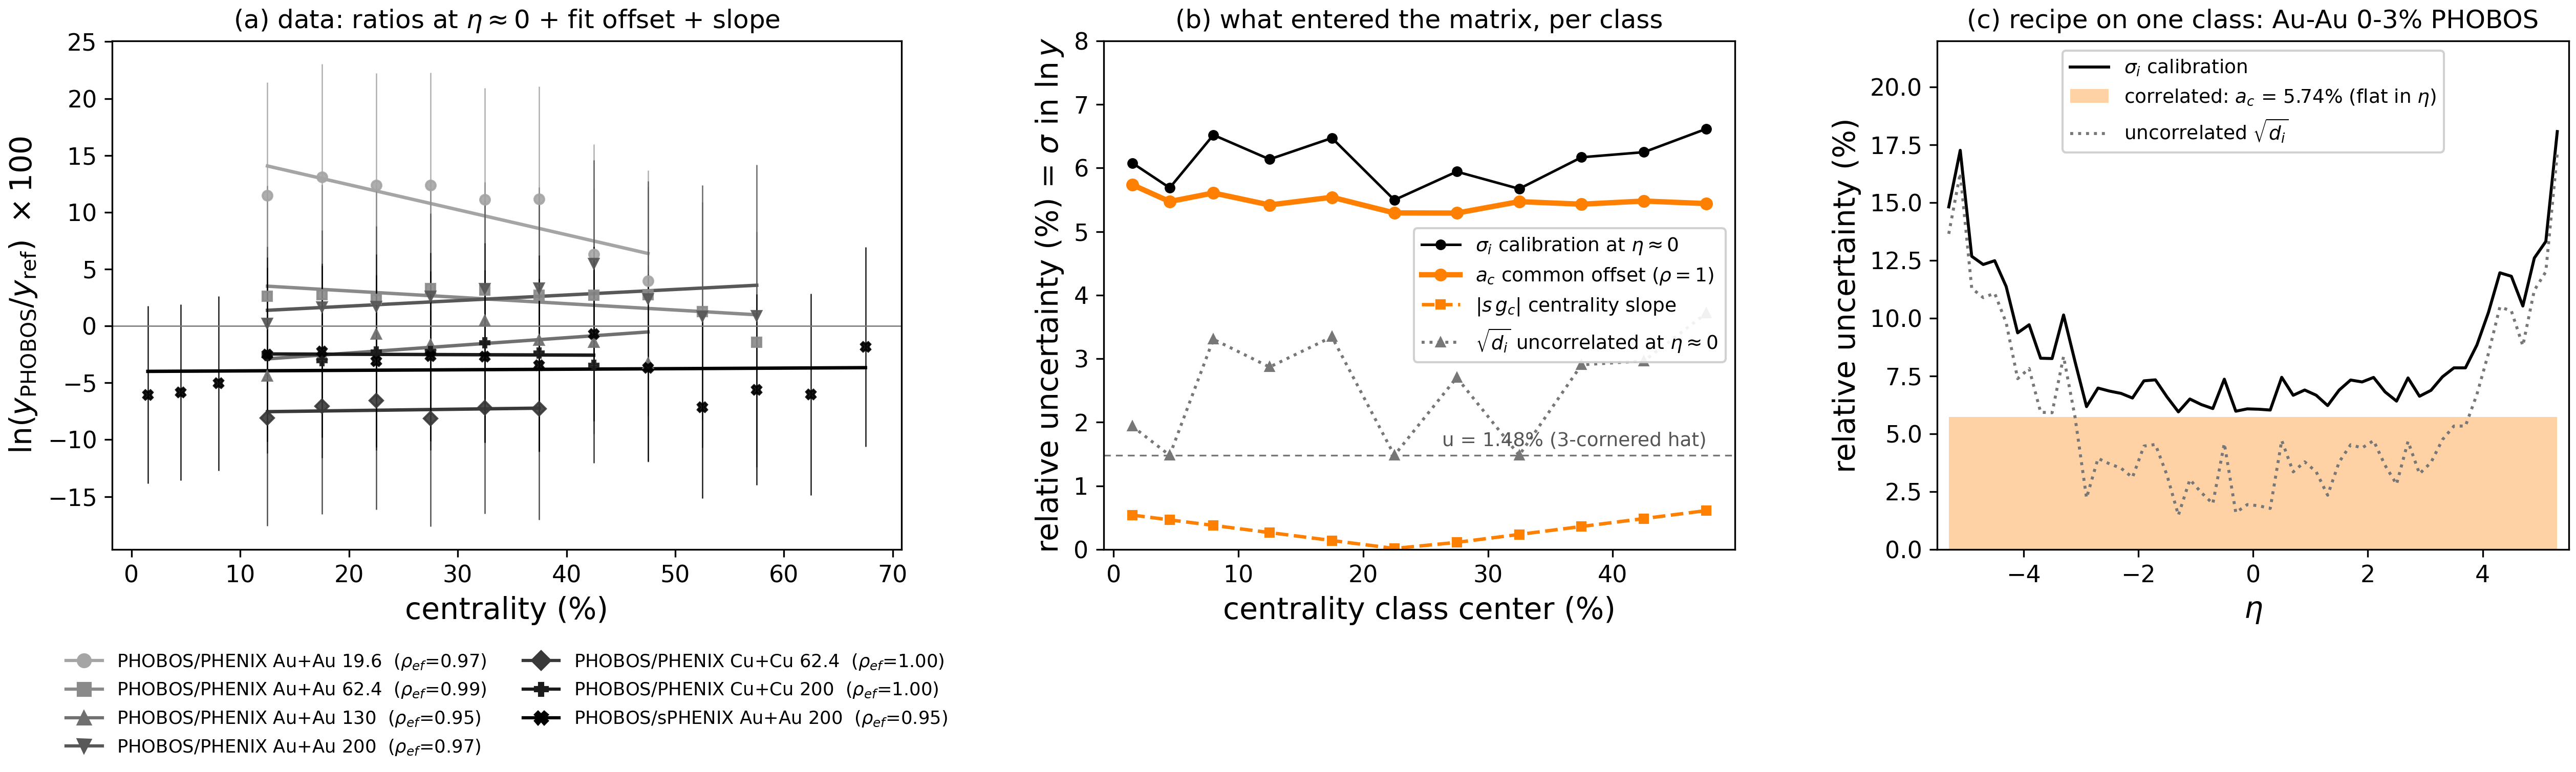
\includegraphics[width=\linewidth]{fig/I1-covariance__covinf__learnphob.png}
\caption{(a) Dados: $\ln(y_{\rm PHOBOS}/y_{\rm ref})$ por classe, com barras $\sigma_{r}$ (soma dos dois detectores) e a reta
ajustada. Os pontos formam retas muito mais estreitas que as barras, ou seja, o erro é quase todo comum às classes.
(b) O que entrou na matriz, por classe: $\sigma_i$ da calibração em $\eta\approx0$, offset comum $a_c$, $|s\,g_c|$ e
$\sqrt{d_i}$. (c) A receita numa classe (0--3\%): $a_c$ é plano em $\eta$, e o crescimento de $\sigma_i$ no $\eta$ frontal vai
todo para a parte não correlacionada.}
\end{figure}

Em todos os conjuntos, $\rho_{\rm ef}=\valRhoMin$--$\valRhoMax$. Os offsets ficam dentro das incertezas (pull rms $\approx0{,}7$). A
inclinação depende da energia: é grande em 19,6\,GeV e pequena de 62,4\,GeV em diante. Em 200\,GeV,
$\beta_{\rm PHOBOS/PHENIX}=\valSlopePHENIX\%$ e $\beta_{\rm PHOBOS/sPHENIX}=\valSlopeSPHENIX\%$, o que dá $s=\valS$.
O terceiro momento dos resíduos padronizados, $-0{,}08\pm0{,}24$, é compatível com zero.

\subsection{Three-cornered hat}
Desvio classe a classe: PHENIX $\valTchPHENIX\%$, \textbf{PHOBOS $\valTchPHOBOS\%$} ($\Rightarrow u$), sPHENIX $\valTchSPHENIX\%$.
As incertezas citadas ficam em 4,7--7,4\%: a parte que muda de classe para classe é uma fração pequena delas.

\subsection{A matriz}
Componentes por classe (em \%; $\sigma$ em log é a incerteza relativa):
\begin{center}\small
\begin{tabular}{@{}l r r r r r r r r@{}}
\toprule
classe (\%) & $c$ & $g_c$ & $\sigma_i(\eta\approx0)$ & $\min_\eta\sigma_i$ & $\max_\eta\sigma_i$ & $a_c$ & $s\,g_c$ & $\sqrt{d_i}(\eta\approx0)$ \\
\midrule
\tabin{tab/classes.tex}
\bottomrule
\end{tabular}
\end{center}

\caixa{orange!10}{\textbf{É uma covariância constante?} Em covariância, essencialmente sim. $a_c$ varia só entre $\valAmin\%$ e
$\valAmax\%$ (média $\valAmean\%$), e $|s\,g_c|\le\valSlopeMax\%$. A matriz é, portanto, $a^2\approx\valAsq$ \emph{somado a todos
os \valNbins{} bins} (um fator de escala comum $1\pm{\approx}\valAmean\%$ em todo o $dN/d\eta$ do PHOBOS), mais a diagonal
restante. O primeiro autovetor do bloco carrega $\valEigOne\%$ da variância, e o segundo só $\valEigTwo\%$.
A \emph{correlação} não é constante, porque $\rho_{ij}\approx a^2/(\sigma_i\sigma_j)$ e $\sigma_i$ cresce no $\eta$ frontal.
Média fora da diagonal: $\valCorrMean$ (mínimo $\valCorrMin$, máximo $\valCorrMax$).}

Correlação entre classes no bin de $\eta\approx0$ (o que os dados de fato restringem):
\begin{center}\footnotesize
\begin{tabular}{@{}l *{11}{r}@{}}
\toprule
\tabin{tab/corr11.tex}
\bottomrule
\end{tabular}
\end{center}
Mínimo $\valCorrEtaMin$ e média $\valCorrEtaMean$. Esses valores ficam abaixo de $\rho_{\rm ef}\approx0{,}97$ porque a variância da
calibração em $\eta\approx0$ ($\sigma_i$) é maior que a parte comum $a_c$ em algumas classes (Sec.~\ref{sec:aberto}).

\begin{figure}[H]
\centering
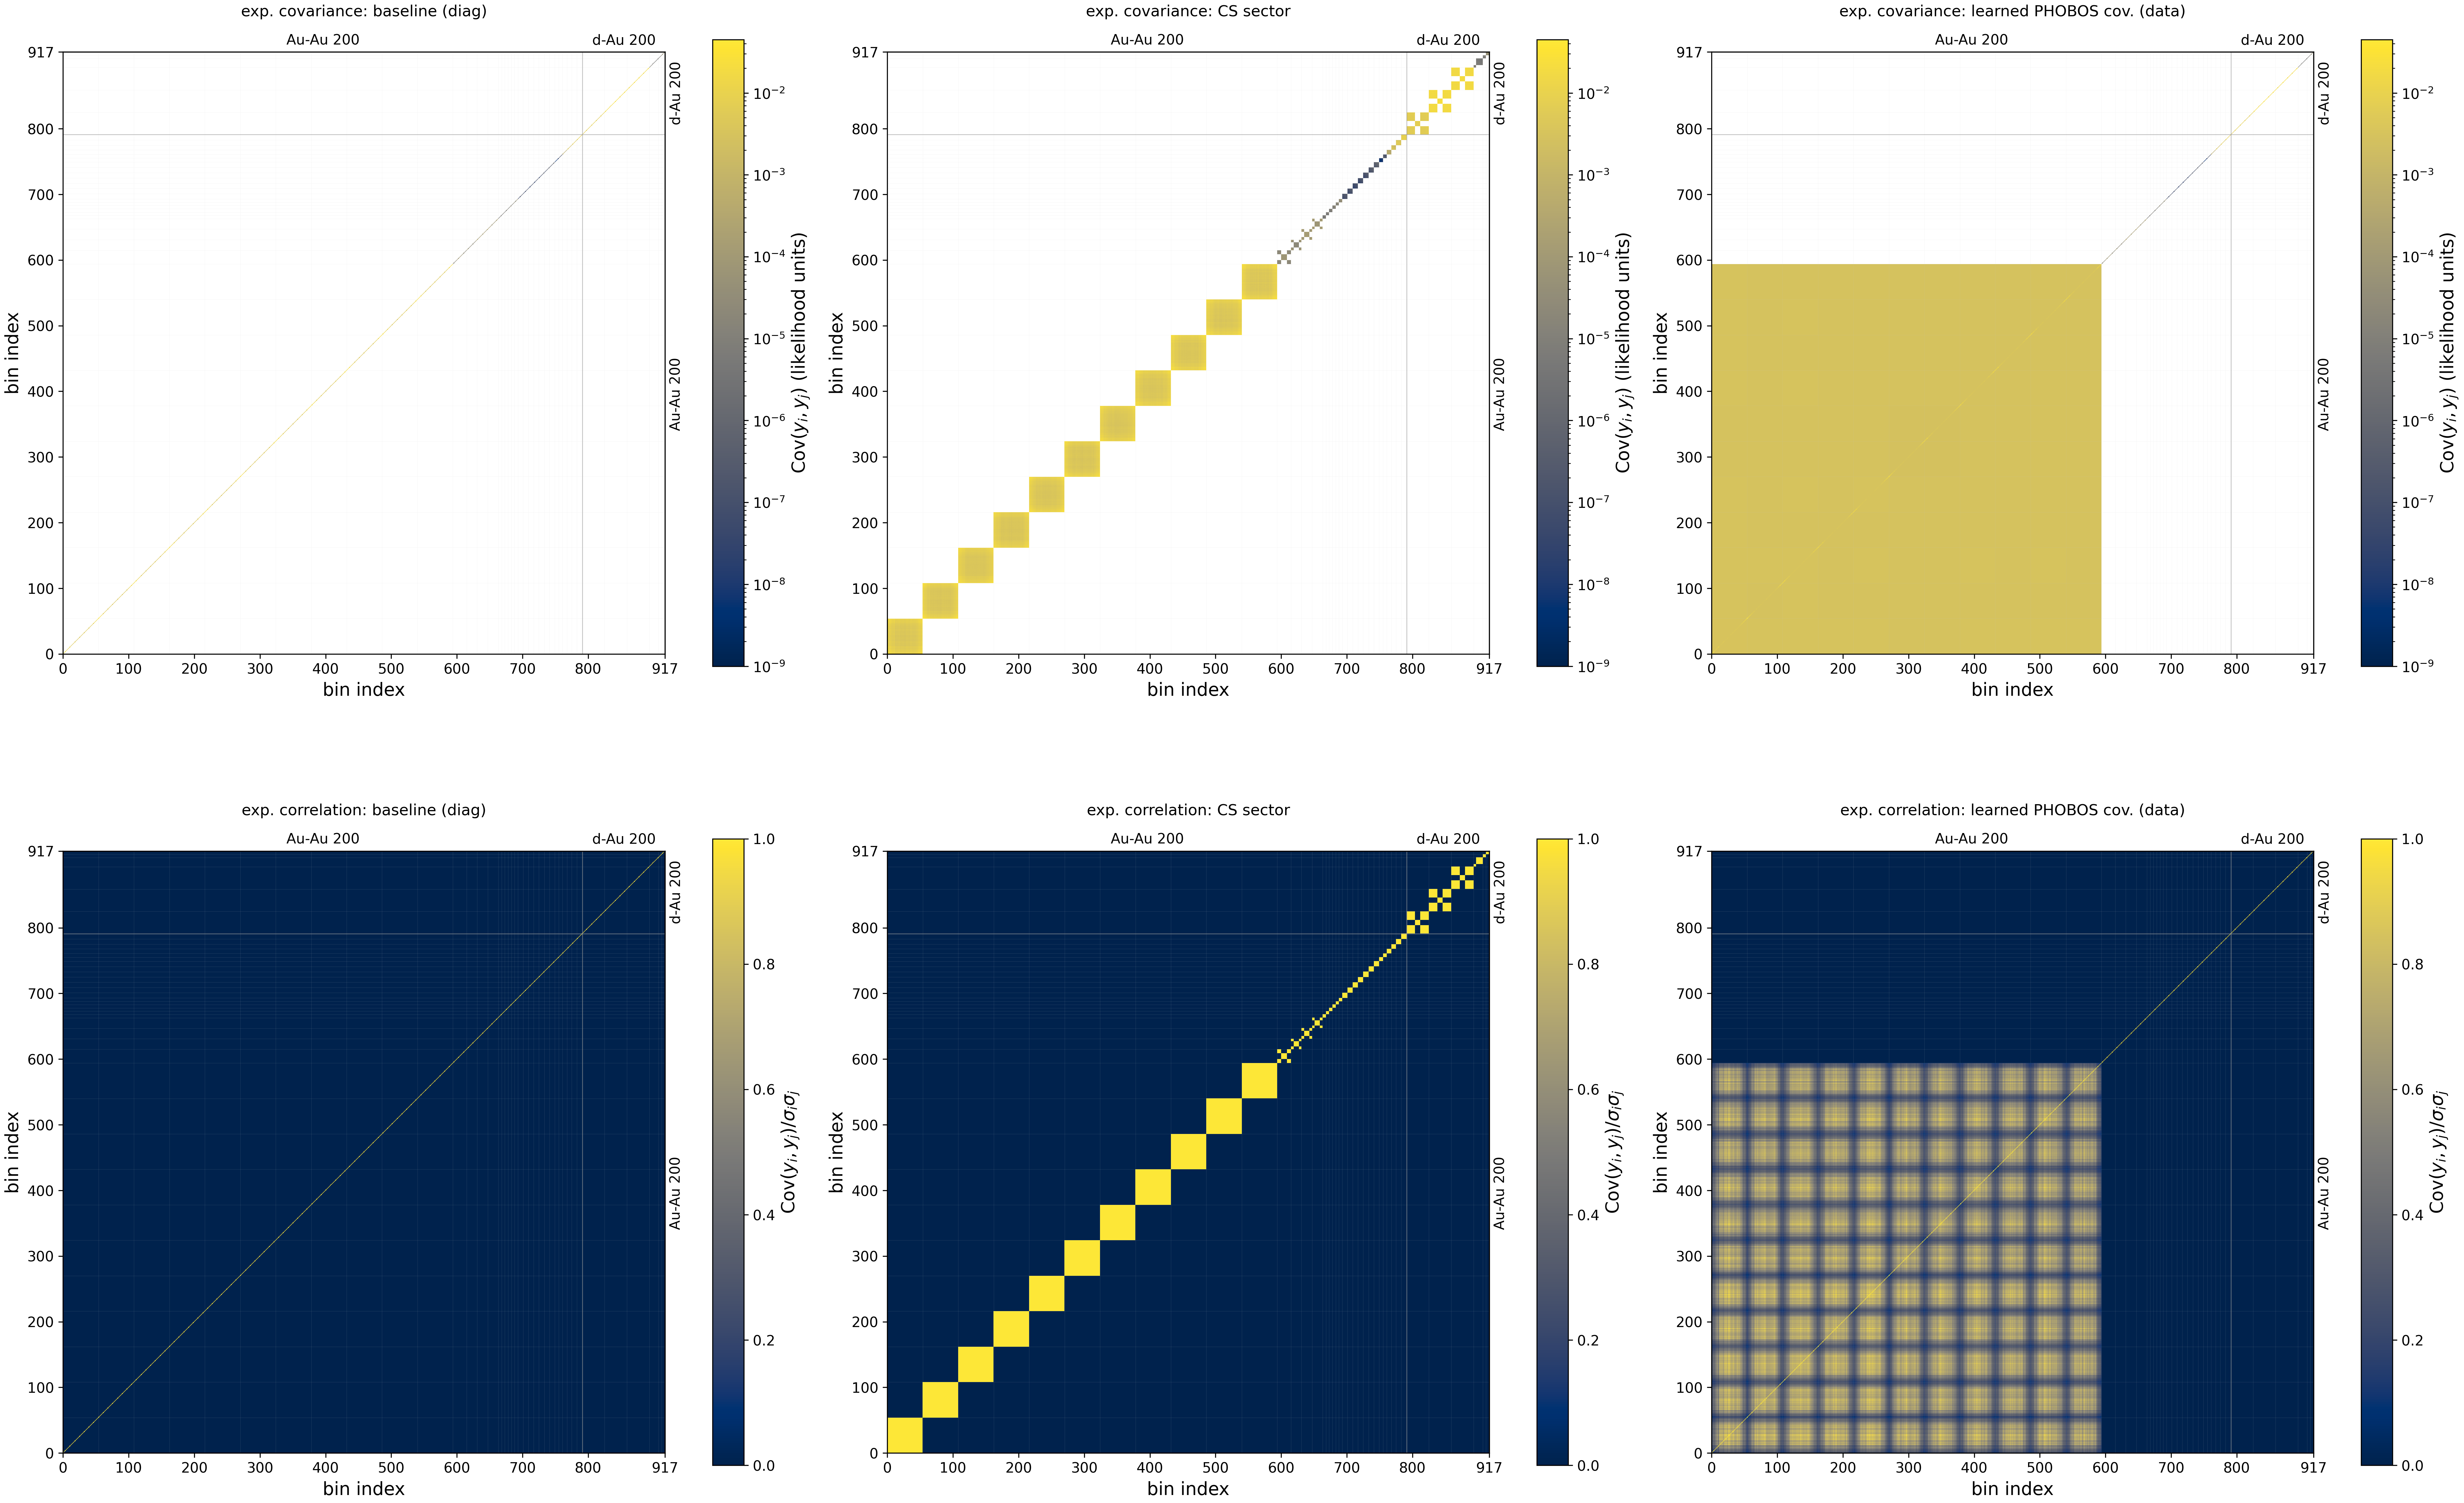
\includegraphics[width=\linewidth]{fig/S2-expcov__covinf__baseline-cs-learnphob.png}
\caption{Covariância (em cima) e correlação (embaixo) experimentais nos 917 bins: baseline, CS sector e o modelo
aprendido (bins 0--593: PHOBOS $dN/d\eta$). As estruturas do CS sector e do modelo aprendido são opostas. O CS sector põe
$\rho=1$ dentro de cada classe (todo $\eta$) e $\rho=0$ entre classes. O modelo aprendido correlaciona as classes, que é o
que os dados mostram, e deixa o $\eta$ frontal quase sem correlação.}
\end{figure}

A matriz completa ($\valNbins\times\valNbins$, em log) está em \arq{I1-covariance__covinf__learnphob__matrix_cov.csv} e em
\arq{..._matrix.npz} (\texttt{cov}, \texttt{corr}, \texttt{sigma}, \texttt{labels}). A Eq.~\eqref{eq:sigma}, com a tabela
acima e os $\sigma_i$ do Apêndice~\ref{ap:bins}, a reproduz exatamente.

\section{O que foi inferido e o que foi suposto}\label{sec:origem}
\begin{center}\small
\begin{tabularx}{\linewidth}{@{}Y l l@{}}
\toprule
ingrediente & origem & valor \\
\midrule
correlação entre classes de centralidade (termo comum) & \textbf{dados}: $\rho_{\rm ef}$ de \valNsets{} conjuntos & $\rho\approx1$ \\
inclinação em centralidade & \textbf{dados}: 200\,GeV, 2 pares & $s=\valS$ \\
parte não correlacionada mínima & \textbf{dados}: three-cornered hat & $u=\valU\%$ \\
\emph{tamanho} do termo comum & \textbf{escolha}: o máximo que a variância da calibração permite & $a_c=\valAmin$--$\valAmax\%$ \\
termo comum plano em $\eta$ & \textbf{hipótese}: só $\eta\approx0$ foi medido & --- \\
variância extra no $\eta$ frontal sem correlação & \textbf{hipótese} & $\sqrt{d_i}$ até ${\sim}20\%$ \\
variância total de cada bin & \textbf{calibração} (JETSCAPE), mantida & $\sigma_i$ \\
\bottomrule
\end{tabularx}
\end{center}
O tamanho do termo comum não pode ser medido assim: diferenças entre detectores só revelam o sistemático
\emph{relativo}. A inferência fixa a \textbf{estrutura} (o erro é comum às classes, com uma pequena parte classe a
classe). A escala vem da variância já usada na calibração.

\section{Uso na calibração}
A partir da matriz, o procedimento é o mesmo de todas as propostas.
\begin{itemize}[nosep]
\item Cadeia: \texttt{bayes\_mcmc\_learned\_phobos.py --u 0.0148 --slope 0.025}, 200 walkers, 20\,000 passos de burn-in e
20\,000 de produção (job Condor 5079): \arq{mcmc/02_14_learned_phobos_normalization/chain-idf-0-learned-phobos-7ec3735f96a8.hdf}.
\item Checagem antes de rodar: \texttt{--check-covariance} (positiva definida, diagonal inalterada, assinatura
\texttt{7ec3735f96a8}, gravada no HDF).
\item Figuras: pastas 01--07 desta proposta, no design system comum, com comparação contra baseline e CS sector.
Efeito no posterior: todos os deslocamentos de mediana ficam abaixo de $1\sigma$ da baseline.
\item Para reaplicar em outro estudo: usar a mesma função com os $\sigma_i$ do estudo. O bloco é identificado pelo nome
\texttt{dNdeta\_eta\_cen\_<lo>\_<hi>\_PHOB}, e os demais bins ficam diagonais.
\end{itemize}

\section{Limitações e pontos em aberto}\label{sec:aberto}
\begin{itemize}[nosep]
\item \textbf{90\% C.L.\ como $1\sigma$?} O $\sigma_i$ da calibração em $\eta\approx0$ (5,5--6,6\%) fica entre o $1\sigma$ do PHOBOS
(${\approx}4{,}6\%$) e o valor em 90\% C.L.\ (${\approx}7{,}5\%$). Se a calibração inflou o PHOBOS, $a_c$ herda a inflação.
\item \textbf{Forma em $\eta$} do termo comum e \textbf{variância frontal}: hipóteses, ainda sem dados.
\item \textbf{Energia:} só a inclinação de 200\,GeV entrou. Em 19,6\,GeV ela é cerca de 4$\times$ maior.
\item \textbf{Independência:} os conjuntos compartilham detectores ($N_{\rm ef}\approx7$). Os ajustes são descritivos, não
uma estimativa conjunta com incerteza.
\end{itemize}

\section*{Arquivos}
\begin{center}\footnotesize
\begin{tabularx}{\linewidth}{@{}l Y@{}}
\toprule
dados entre detectores & \arq{study_nongaussian_systematics/data/midrapidity_dndeta.csv}, \arq{sphenix_dndeta_vs_eta.csv}, \arq{README_data.md} \\
estudo original (fatia 2a) & \arq{study_nongaussian_systematics/fatia2a/} (\arq{fatia2a_normalizacao.py}, \arq{results.json}) \\
matriz & \arq{experimental_learned_covariance.py} \\
números deste documento & \arq{mcmc/scripts/paper_figures/info_covariance.py} $\rightarrow$ \arq{I1-covariance__covinf__learnphob.json}; tabelas: \arq{info_covariance_tex.py} \\
fonte deste documento & \arq{mcmc/scripts/paper_figures/recipes/I1-covariance__covinf/} \\
\bottomrule
\end{tabularx}
\end{center}

\appendix
\section{Todas as comparações usadas}\label{ap:dados}
{\footnotesize
\begin{longtable}{@{}l r r r r r@{}}
\toprule
classe (\%) & PHOBOS $|\eta|<1$ $\pm$ sys 90\% & PHOBOS $\to|\eta|<0{,}3$ & $\sigma_{\rm PHOBOS}$ ($1\sigma$) & referência $\pm\sigma$ & $r$ (\%) $\pm\sigma_r$ \\
\endhead
\tabin{tab/dados.tex}
\bottomrule
\end{longtable}}

\section{Incertezas da calibração por bin}\label{ap:bins}
$\sigma_i$ em \% (log), por bin de $\eta$ (linhas) e classe de centralidade (colunas). Com a tabela de $a_c$, $s$, $g_c$ e a
Eq.~\eqref{eq:sigma}, estes valores determinam a matriz inteira.
{\scriptsize
\begin{longtable}{@{}r *{11}{r}@{}}
\toprule
\tabin{tab/bins_sigma.tex}
\bottomrule
\end{longtable}}

Parte não correlacionada $\sqrt{d_i}$ em \%:
{\scriptsize
\begin{longtable}{@{}r *{11}{r}@{}}
\toprule
\tabin{tab/bins_sqrtd.tex}
\bottomrule
\end{longtable}}

\end{document}
